\begin{figure*}[tbh]
    \centering
    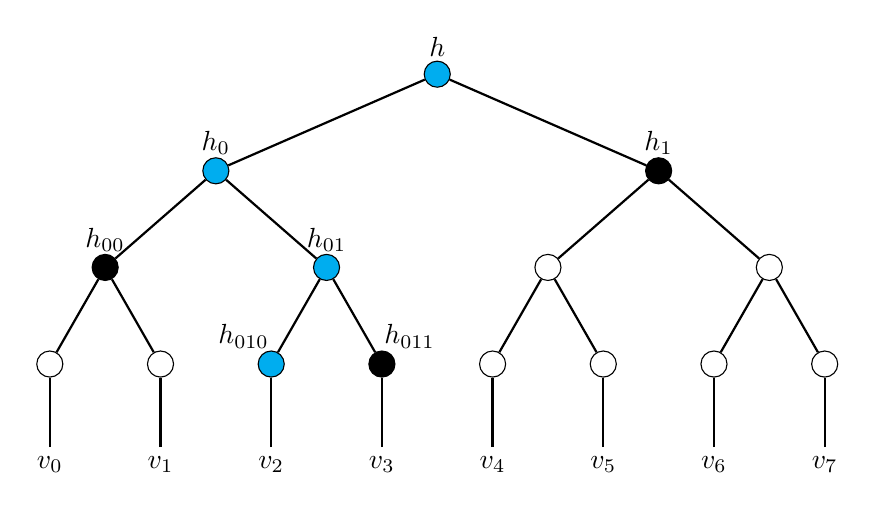
\begin{tikzpicture}[par/.style={sloped,fill=white,inner sep=-.4ex}]
    \tikzstyle{circ} = [circle, draw]
    \tikzstyle{path} = [circle, draw, fill=cyan]
    \tikzstyle{copath} = [circle, draw, fill=black]
        \node[path] (root) {};
        % level 1
        \node[path,below=3em,xshift=-8em] (l) at (root) {};
        \node[copath,below=3em,xshift=8em] (r) at (root) {};
        \draw[-,thick] (l) -- (root);
        \draw[-,thick] (r) -- (root);
        % level 2
        \node[copath,below=3em,xshift=-4em] (ll) at (l) {};
        \node[path,below=3em,xshift=4em] (lr) at (l) {};
        \draw[-,thick] (ll) -- (l);
        \draw[-,thick] (lr) -- (l);
        \node[circ,below=3em,xshift=-4em] (rl) at (r) {};
        \node[circ,below=3em,xshift=4em] (rr) at (r) {};
        \draw[-,thick] (rl) -- (r);
        \draw[-,thick] (rr) -- (r);
        % level 3
        \node[circ,below=3em,xshift=-2em] (lll) at (ll) {};
        \node[circ,below=3em,xshift=2em] (llr) at (ll) {};
        \draw[-,thick] (lll) -- (ll);
        \draw[-,thick] (llr) -- (ll);
        \node[path,below=3em,xshift=-2em] (lrl) at (lr) {};
        \node[copath,below=3em,xshift=2em] (lrr) at (lr) {};
        \draw[-,thick] (lrl) -- (lr);
        \draw[-,thick] (lrr) -- (lr);
        \node[circ,below=3em,xshift=-2em] (rll) at (rl) {};
        \node[circ,below=3em,xshift=2em] (rlr) at (rl) {};
        \draw[-,thick] (rll) -- (rl);
        \draw[-,thick] (rlr) -- (rl);
        \node[circ,below=3em,xshift=-2em] (rrl) at (rr) {};
        \node[circ,below=3em,xshift=2em] (rrr) at (rr) {};
        \draw[-,thick] (rrl) -- (rr);
        \draw[-,thick] (rrr) -- (rr);
        % leaves
        \node[below=3em] (0) at (lll) {$v_0$};
        \draw[-,thick] (0) -- (lll);
        \node[below=3em] (1) at (llr) {$v_1$};
        \draw[-,thick] (1) -- (llr);
        \node[below=3em] (2) at (lrl) {$v_2$};
        \draw[-,thick] (2) -- (lrl);
        \node[below=3em] (3) at (lrr) {$v_3$};
        \draw[-,thick] (3) -- (lrr);
        \node[below=3em] (4) at (rll) {$v_4$};
        \draw[-,thick] (4) -- (rll);
        \node[below=3em] (5) at (rlr) {$v_5$};
        \draw[-,thick] (5) -- (rlr);
        \node[below=3em] (6) at (rrl) {$v_6$};
        \draw[-,thick] (6) -- (rrl);
        \node[below=3em] (7) at (rrr) {$v_7$};
        \draw[-,thick] (7) -- (rrr);
        %%% labels
        % path
        \node[yshift=1em] at (root) {$h$};
        \node[yshift=1em] at (l) {$h_0$};
        \node[yshift=1em] at (lr) {$h_{01}$};
        \node[yshift=1em,xshift=-1em] at (lrl) {$h_{010}$};
        % copath
        \node[yshift=1em] at (r) {$h_1$};
        \node[yshift=1em] at (ll) {$h_{00}$};
        \node[yshift=1em,xshift=1em] at (lrr) {$h_{011}$};
    \end{tikzpicture}
    \caption{Each node in a Merkle tree consists of a hash of its children. The root $h$ is a commitment to the vector $(v_0, v_1, \dots, v_7)$ consisting of the leaves. To open the leaf at position 2, a prover provides the value $v_2$ and an opening proof $\pi$ consisting of the copath (black nodes) $(h_{011}, h_{00}, h_{1})$. The proof $\pi$ is checked by using its contents to recompute the root $h'$ starting with $v_2$, then checking that $h = h'$.
    In a naysayer proof system, the prover provides $\pi$ along with a ``verification trace'': the blue nodes $\com = (h_{010}, h_{01}, h_{0})$. A naysayer can point out an error at a particular point of the trace, e.g., $h_{01}$, which the naysayer verifier checks by computing a single hash, e.g., $H(h_{010}, h_{011}) \stackrel{?}{=} h_{01}$.}
    \label{fig:merkle-diagram}
\end{figure*}